% !TEX root =../thesis-letomes.tex

\chapter{Physical Modelling}
We need a chapter to formulate our hypotheses, and generally give a before-the-fact run-down of what the project and report will be like.

\section{CM-Centered Restricted 3-Body System (C-R3B), Earth-Moon}
The center-of-mass-centered 3-body system (C-R3B) with the Earth and Moon was explored in \cite{Saxe2015}. We will shortly present the final nondimensionalized equations of motion here for reference, since we have done much analysis on the Earth-Moon system in this project as well.

\subsection{C-R3B Equations of Motion}

\begin{empheq}[box=\widefbox]{align}
\label{eq:Xdot}
\dot{X} = P_x + Y
\end{empheq}

\begin{empheq}[box=\widefbox]{align}
\label{eq:Ydot}
\dot{Y} = P_Y - X
\end{empheq}

\begin{empheq}[box=\widefbox]{align}
\label{eq:Pdot_X}
\dot{P}_X = P_Y - \dfrac{(1-k)(X+k)}{((X+k)^2+Y^2)^{3/2}} - \dfrac{k(X-1+k))}{((X-1+k))^2+Y^2)^{3/2}}
\end{empheq}

\begin{empheq}[box=\widefbox]{align}
\label{eq:Pdot_Y}
\dot{P}_Y = -P_X - \dfrac{(1-k)Y}{((X+k)^2+Y^2)^{3/2}} - \dfrac{k Y}{((X-1+k))^2+Y^2)^{3/2}}
\end{empheq}
where \(T\), \(X\), \(Y\), \(P_x\) and \(P_y\) are our dimensionless variables for time, positions, generalized impulse, and \(k=\dfrac{M_{\Moon}}{M_{\Earth} + M_{\Moon}}\), that is the ratio of Moon's mass to the total Moon and Earth mass.

\subsection{C-R3B Numerical Algorithms}
Both a symplectic Euler and symplectic Störmer-Verlet (also symplectic) were performed, see \cite{Saxe2015} for details.


\section{Heliocentric Restricted 4-Body System (H-R4B), Sun-Earth-Mars}
Simulating orbit from Earth to Mars requires a new model with at least four bodies: Sun, Earth, Mars and the Spacecraft. The coordinate system will be heliocentric and in spherical coordinates, and restricted meaning that the mass of the spacecraft is considered negligible compared to compared to the celestial masses, so we call this system the ``Heliocentric Restricted N-Body'' system. We will derive the equations of motion of the spacecraft by using Hamilton's equations, which naturally gives us a set of coupled first-order differential equations, and a set of conserved quantities as ``generalized momenta''.

\subsection{Spherical Coordinate System}
We adopt the spherical coordinate system which customary in astrodynamics. The conventions used is in \cref{fig:3D_Spherical}.

\begin{figure}[ht]
    \centering
    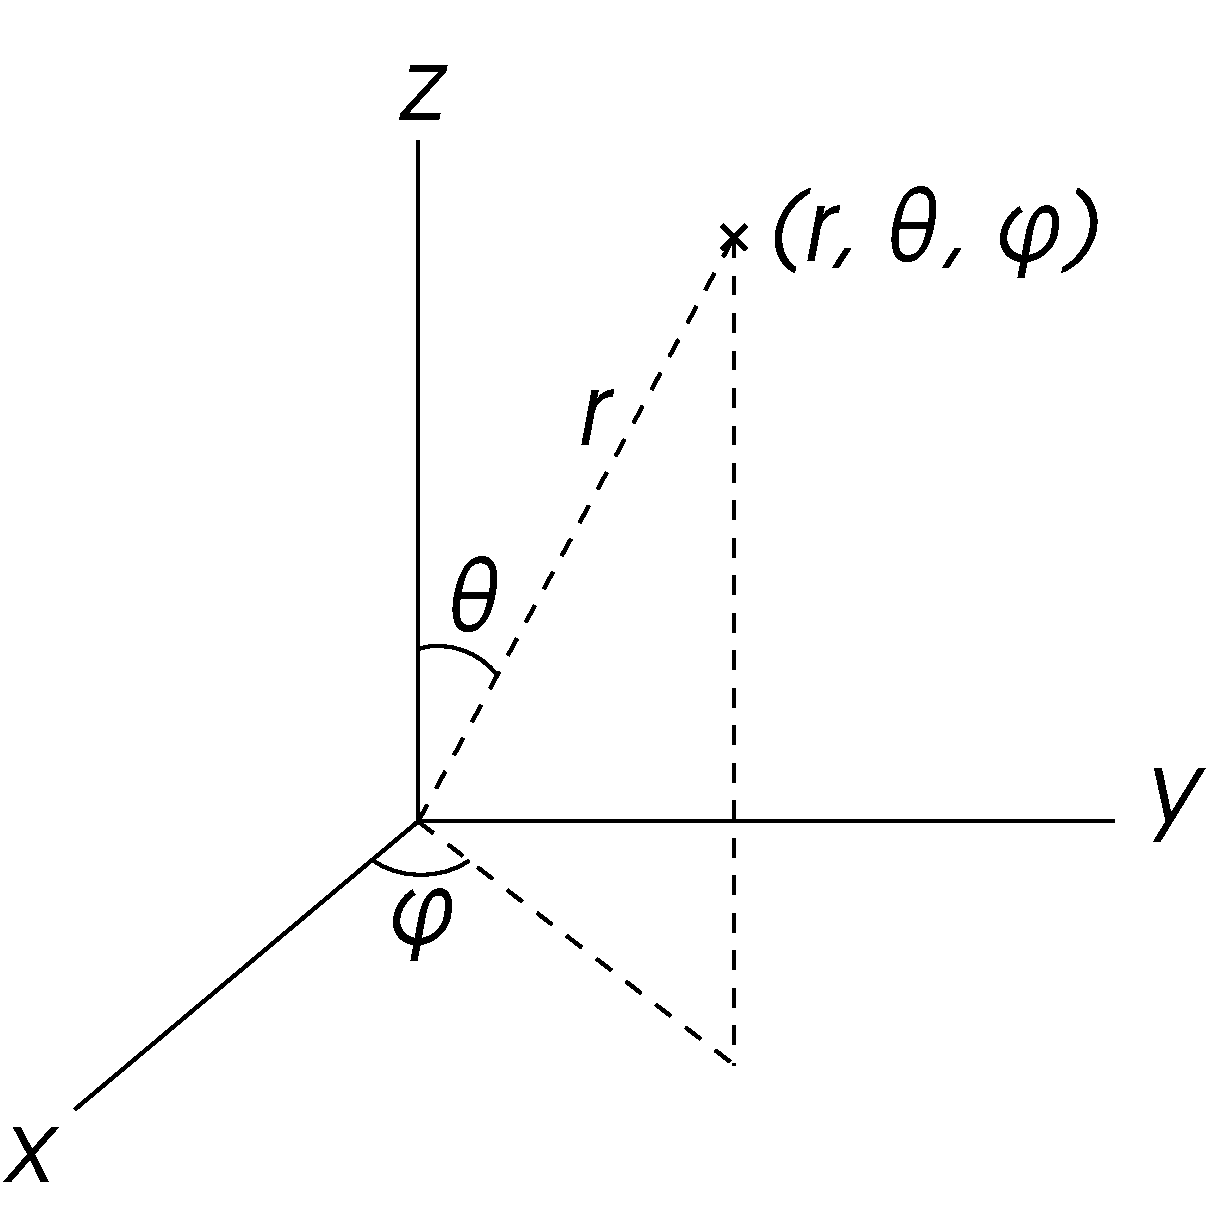
\includegraphics[width=0.50\linewidth]{fig/3D_Spherical2}
    \caption{Spherical coordinates \((r, \theta, \phi)\). Radial distance \(r\), polar angle \(\theta\) (theta), and azimuthal angle \(\phi\) (phi). In our heliocentric system the sun is assumed to be stationary at the origin. Source: \cite{WikiSpherical}.}
    \label{fig:3D_Spherical}
\end{figure}

And the coordinate transform equations to and from the cartesian coordinate system are:

\begin{align}
    x &= r \sin{\theta}\cos{\phi}, \label{eq:x(q)} \\
    y &= r \sin{\theta}\sin{\phi}, \label{eq:y(q)}\\
    z &= r \cos{\theta}, \label{eq:z(q)}
\end{align}

and

\begin{align}
    r &= \sqrt{x^2 + y^2 + z^2}, \label{eq:r(x,y,z)}\\
    \theta &= \arccos{\frac{z}{r}}, \label{eq:theta(x,y,z)}\\
    % \arctan{\frac{y}{x}}, \qquad \theta  \in [0, 2\pi]
    \phi &= 
    \begin{cases}
    \arctan{\frac{y}{x}} & \text{if \(x \geq 0\) \qquad \qquad \ \ \ (Q1, Q4),}
    \\
    \arctan{\frac{y}{x}}+\pi & \text{if \(x \leq 0,\ y \geq 0\) \qquad (Q2),}
    \\
    \arctan{\frac{y}{x}}-\pi & \text{if \(x \leq 0,\ y \leq 0\) \qquad (Q3).}
    \end{cases} \label{eq:phi(x,y,z)}
\end{align}

where \(r \in [0, \infty]\), \(\theta \in [0, \pi]\) and \(\phi \in [0, 2\pi]\).

For the calculation of kinetic in the next section we will need the position vector, unit vectors in spherical coordinates, and the Jacobians.

The position vector in spherical coordinates is
\begin{align}
    \vec{r}(r, \theta, \phi) &= x \xhat + y \yhat + z \zhat \\
    \Leftrightarrow \vec{r}(r, \theta, \phi) &= r \sin{\theta}\cos{\phi} \xhat + r \sin{\theta}\sin{\phi} \yhat + r \cos{\theta} \zhat. \label{eq:position-vec-spherical}
\end{align}

The various coordinate derivatives of the position vector is
\begin{align}
    \pd{\vec{r}}{r} &= \sin{\theta}\cos{\phi} \xhat + \sin{\theta}\sin{\phi} \yhat + \cos{\theta} \zhat \quad &\text{and} \quad &\left| \pd{\vec{r}}{r} \right| = 1 \label{eq:position-derived-r} \\
    \pd{\vec{r}}{\theta} &= r \cos{\theta}\cos{\phi} \xhat + r \cos{\theta}\sin{\phi} \yhat - r \sin{\theta} \zhat \quad &\text{and} \quad &\left| \pd{\vec{r}}{\theta} \right| = r \label{eq:position-derived-theta} \\
    \pd{\vec{r}}{\phi} &= -r\sin{\theta}\sin{\phi} \xhat + r\sin{\theta}\cos{\phi} \zhat \quad &\text{and} \quad &\left| \pd{\vec{r}}{\phi} \right| = r\sin{\theta} \label{eq:position-derived-phi}
\end{align}

So the unit vectors in spherical coordinates are
\begin{align}
    \rhat = \dfrac{\pd{\vec{r}}{r}}{\left| \pd{\vec{r}}{r} \right| } &= \sin{\theta}\cos{\phi} \xhat + \sin{\theta}\sin{\phi} \yhat + \cos{\theta} \zhat \label{eq:r-hat}\\
    \thetahat = \dfrac{\pd{\vec{r}}{\theta}}{\left| \pd{\vec{r}}{\theta} \right| } &= \cos{\theta}\cos{\phi} \xhat + \cos{\theta}\sin{\phi} \yhat - \sin{\theta} \zhat \label{eq:theta-hat}\\
    \phihat = \dfrac{\pd{\vec{r}}{\phi}}{\left| \pd{\vec{r}}{\phi} \right| } &= -\sin{\phi} \xhat + \cos{\phi} \zhat \label{eq:phi-hat}
\end{align}

\subsection{H-R4B Equations of Motion}
We will follow the 5-step process of arriving at Hamilton's equations outlined in \cref{apx:hamiltons}.

\subsubsection{Step 1: Lagrangian \(L\)}
The kinetic energy of the system is
\begin{align}
    T = \frac{1}{2} m_s v^2.
\end{align}

In general the total derivative of a vector is:

\begin{align}
    \vec{v} &= \od{\vec{r}}{t} = \sum\limits_{j} \pd{\vec{r}}{q_j} \od{q_j}{t}, \\
      &= \sum\limits_{j} \left|\pd{\vec{r}}{q_j}\right| \frac{\pd{\vec{r}}{q_j}}{\left|\pd{\vec{r}}{q_j}\right|} \od{q_j}{t}, \\
      &= \sum\limits_{j} \left|\pd{\vec{r}}{q_j}\right| \od{q_j}{t} \unitvector{q}_j, \\
      &= \sum\limits_{j} \left|\pd{\vec{r}}{q_j}\right| \dot{q_j} \unitvector{q}_j,
    \end{align}

where we have used that a unit vector for any coordinate system is \(\frac{\pd{\vec{r}}{q_j}}{\left|\pd{\vec{r}}{q_j}\right|} = \unitvector{q}_j\).
We can now use the derivatives of the position vector we found earlier in \cref{eq:position-derived-r,eq:position-derived-theta,eq:position-derived-phi}, to substitute for \(\left|\pd{\vec{r}}{q_j}\right|\). We don't have to substitute in \(\unitvector{q}_j\) since our unit vectors are orthogonal, so they will yield either 0 or 1 when we square \(v\). So for the spherical coordinates we get:

\begin{align}
    \vec{v} = \dot{r}\rhat + r\dot{\theta}\thetahat + r\sin{\theta}\,\dot{\phi}\phihat
\end{align}

so

\begin{align}
    v^2 = \dot{r}^2 + r^2\dot{\theta}^2 + r^2\sin^2{\theta}\,\dot{\phi}^2
\end{align}

so we get

\begin{align}
    T = \frac{1}{2} m_s (\dot{r}^2 + r^2\dot{\theta}^2 + r^2\sin^2{\theta}\,\dot{\phi}^2).
\end{align}

The gravitational potential is \todoref{find some non-wikipedia reference here}

\begin{align}
    V = -G m_s \sum\limits_{k} \frac{M_k}{\left| \vec{r} - \vec{r_k} \right|},
\end{align}
where \(i\) denotes the celestial bodies acting on the spacecraft, i.e. in our system Sun, Earth and Mars.

So we finally get the Lagrangian

\begin{align}
    L &= T - V \\
    \Leftrightarrow L &= \frac{1}{2} m_s (\dot{r}^2 + r^2\dot{\theta}^2 + r^2\sin^2{\theta}\,\dot{\phi}^2) + G m_s \sum\limits_{k} \frac{M_k}{\left| \vec{r} - \vec{r_k} \right|}
\end{align}

\subsubsection{Step 2: Generalized Momenta \(p_j\)}
\begin{align}
    p_r &= \pd{L}{\dot{r}} = m_s \dot{r} \label{eq:pr} \\
    p_\theta &= \pd{L}{\dot{\theta}} = m_s r^2 \dot{\theta} \label{eq:ptheta} \\
    p_\phi &= \pd{L}{\dot{\phi}} = m_s r^2 \sin^2{\theta} \dot{\phi} \label{eq:pphi}
\end{align}

\subsubsection{Step 3: \(\dot{q} = \dot{q}_j(\vec{q}, \vec{p}, t)\)}
\begin{align}
    \dot{r} &= \frac{p_r}{m_s} \\
    \dot{\theta} &= \frac{p_\theta}{m_s r^2} \\
    \dot{\phi} &= \frac{p_\phi}{m_s r^2 \sin^2{\theta}}
\end{align}

We can now rewrite \(L\) to make it independent of \(\dot{q}\) by substituting the expressions above:

\begin{align}
    T &= \frac{1}{2} m_s (\dot{r}^2 + r^2\dot{\theta}^2 + r^2\sin^2{\theta}\,\dot{\phi}^2) \\
    &= \frac{1}{2} m_s \left(\frac{p_r^2}{m_s^2} + r^2\frac{p_\theta^2}{m_s^2 r^4} + r^2\sin^2{\theta}\frac{p_\phi^2}{m_s^2 r^4 \sin^4{\theta}} \right) \\
    &= \frac{p_r^2}{2 m_s} + \frac{p_\theta^2}{2 m_s r^2} + \frac{p_\phi^2}{2 m_s r^2 \sin^2{\theta}} \\
\end{align}

So we have

\begin{align}
    L = \frac{p_r^2}{2 m_s} + \frac{p_\theta^2}{2 m_s r^2} + \frac{p_\phi^2}{2 m_s r^2 \sin^2{\theta}} + G m_s \sum\limits_{k} \frac{M_k}{\left| \vec{r} - \vec{r_k} \right|}
\end{align}

\subsubsection{Step 4: Hamiltonian \(H\)}
\begin{align}
    H(\vec{q}, \vec{p}, t) &= \sum\limits_{j}p_j \dot{q_j} - L \\
    &= \sum\limits_{j}p_j \dot{q_j}(\vec{q}, \vec{p}, t) - L \\
    &= p_r \frac{p_r}{m_s} + p_\theta \frac{p_\theta}{m_s r^2} + p_\phi + \frac{p_\phi}{m_s r^2 \sin^2{\theta}} \nonumber \\
    &- \left( \frac{p_r^2}{2 m_s} + \frac{p_\theta^2}{2 m_s r^2} + \frac{p_\phi^2}{2 m_s r^2 \sin^2{\theta}} + G m_s \sum\limits_{k} \frac{M_k}{\left| \vec{r} - \vec{r_k} \right|} \right) \\
    \Leftrightarrow H &= \frac{p_r^2}{2 m_s} + \frac{p_\theta^2}{2 m_s r^2} + \frac{p_\phi^2}{2 m_s r^2 \sin^2{\theta}} - G m_s \sum\limits_{k} \frac{M_k}{\left| \vec{r} - \vec{r_k} \right|}
\end{align}

At this point we want to expand the expression \(\left| \vec{r} - \vec{r_k} \right|\) in anticipation of needing to differentiate \(H\) with respect to the coordinates. Using the equations for the \(x, y, z\) coordinates \cref{eq:x(q),eq:y(q),eq:z(q)} we get

\begin{align}
    d_k = \left|\vec{r} - \vec{r}_k \right| &= \sqrt{(x-x_k)^2 + (y-y_k)^2 + (z-z_k)^2}
\end{align}
and
\begin{align}
    (x-x_k)^2 &= (r\sin{\theta}\cos{\phi} - r\sin{\theta}\cos{\phi})^2 \nonumber \\
    &= \tikz[baseline]{
        \node[fill=orange!20,anchor=base]
        {\(r^2\sin^2{\theta}\cos^2{\phi}\)}
    } + \tikz[baseline]{
        \node[fill=red!20,anchor=base]
        {\(r_k^2\sin^2{\theta_k}\cos^2{\phi_k}\)}
    } - 2r r_k \sin{\theta}\sin{\theta_k}\cos{\phi}\cos{\phi_k} \label{eq:x-dist-squared} \\
    (y-y_k)^2 &= (r\sin{\theta}\sin{\phi} - r\sin{\theta}\sin{\phi})^2 \nonumber \\
    &= \tikz[baseline]{
        \node[fill=orange!20,anchor=base]
        {\(r^2\sin^2{\theta}\sin^2{\phi}\)}
    } + \tikz[baseline]{
        \node[fill=red!20,anchor=base]
        {\(r_k^2\sin^2{\theta_k}\sin^2{\phi_k}\)}
    } - 2r r_k \sin{\theta}\sin{\theta_k}\sin{\phi}\sin{\phi_k} \label{eq:y-dist-squared} \\
    (z-z_k)^2 &= (r\cos{\theta} - r\cos{\theta})^2 \nonumber \\
    &= \tikz[baseline]{
        \node[fill=orange!20,anchor=base]
        {\(r^2\cos^2{\theta}\)}
    } + \tikz[baseline]{
        \node[fill=red!20,anchor=base]
        {\(r_k^2\cos^2{\theta_k}\)}
    } - 2r r_k \cos{\theta}\cos{\theta_k}. \label{eq:z-dist-squared}
\end{align}
Now adding all three \cref{eq:x-dist-squared,eq:y-dist-squared,eq:z-dist-squared} the orange terms add to \(r^2\) and the red terms add to \(r_k^2\) and we get

\begin{align}
    d_k &= \sqrt{
        \tikz[baseline]{\node[fill=orange!20,anchor=base]{\(r^2\)}}
        + \tikz[baseline]{\node[fill=red!20,anchor=base]{\(r_k^2\)}}
        -2r r_k(\cos{\theta}\cos{\theta_k}+\sin{\theta}\sin{\theta_k}(
            \tikz[baseline]{\node[fill=blue!20,anchor=base]{
                \(\cos{\phi}\cos{\phi_k} + \sin{\phi}\sin{\phi_k}\)}}
        ))
    } \\
    &= \sqrt{(r - r_k)^2(\cos{\theta}\cos{\theta_k}+\sin{\theta}\sin{\theta_k}(\cos{\phi - \phi_k}))},
\end{align}
where the blue factor was simplified using the sum rule \cite{WeissteinTrig}: \\
\(\cos{\alpha}\cos{\beta} + \sin{\alpha}\sin{\beta} = cos{\alpha-\beta}\).

So we can finally express \(H\) as
\begin{equation}
    \begin{aligned}
        H &= \frac{p_r^2}{2 m_s} + \frac{p_\theta^2}{2 m_s r^2} + \frac{p_\phi^2}{2 m_s r^2 \sin^2{\theta}} \\
        &- G m_s \sum\limits_{k} \frac{M_k}{\sqrt{(r - r_k)^2\left[\cos{\theta}\cos{\theta_k}+\sin{\theta}\sin{\theta_k}\cos{(\phi - \phi_k})\right]}}
    \end{aligned}
\end{equation}

\subsubsection{Step 5: Hamilton's Equations}
\begin{align}
    \dot{r} = \pd{H}{p_r} &= \frac{p_r}{m_s} \label{eq:rdot} \\[0.3cm]
    \dot{\theta} = \pd{H}{p_\theta} &= \frac{p_\theta}{m_s r^2} \label{eq:thetadot} \\[0.3cm]
    \dot{\phi} = \pd{H}{p_\phi} &= \frac{p_\phi}{m_s r^2 \sin^2{\theta}} \label{eq:phidot}  \\[0.3cm]
    \begin{split}
        \dot{p}_r = -\pd{H}{r} &= \frac{p_\theta^2}{m_s r^3} + \frac{p_\phi^2}{m_s r^3 \sin^2{\theta} } \\
        &+ G m_s \sum\limits_{k} M_k \frac{-\left[r - r_k \left(\cos{\theta}\cos{\theta_k} + \sin{\theta}\sin{\theta_k}\cos{(\phi - \phi_k)}\right) \right]}{\left[(r - r_k)^2 \left(\cos{\theta}\cos{\theta_k} + \sin{\theta}\sin{\theta_k}\cos{(\phi - \phi_k)} \right) \right]^{3/2}} \label{eq:prdot}
    \end{split} \\[0.3cm]
    \begin{split}
        \dot{p}_\theta = -\pd{H}{\theta} &= \frac{p_\phi^2}{m_s r^2 \sin^2{\theta} \tan{\theta}} \\
        &+ G m_s \sum\limits_{k} M_k \frac{r r_k \left[-\sin{\theta}\cos{\theta_k} + \cos{\theta}\sin{\theta_k}\cos{(\phi - \phi_k)} \right]}{\left[(r - r_k)^2 \left(\cos{\theta}\cos{\theta_k} + \sin{\theta}\sin{\theta_k}\cos{(\phi - \phi_k)} \right) \right]^{3/2}} \label{eq:pthetadot}
    \end{split} \\[0.3cm]
    \begin{split}
        \dot{p}_\phi = -\pd{H}{\phi} &= G m_s \sum\limits_{k} M_k \frac{- r r_k \sin{\theta}\sin{\theta_k}\sin{(\phi - \phi_k)}}{\left[(r - r_k)^2 \left(\cos{\theta}\cos{\theta_k} + \sin{\theta}\sin{\theta_k}\cos{(\phi - \phi_k)} \right) \right]^{3/2}} \label{eq:pphidot}
    \end{split}
\end{align}

Those are our equations of motion. However before we try to solve them, we will remove all units.

\subsection{H-R4B Equations Nondimensionalized}
We will now choose suitable characteristic units, which has a number of benefits:
\begin{itemize}
    \item The equations gets slightly simplified
    \item The order of the effects of different forces in the system becomes more apparent.
    \item Many of the calculations in numerical algorithms happens at an order of about 1. 
\end{itemize}

The characteristic units are chosen as:
\begin{align}
    \text{Unit length: } k_r &= a_{\Earth}\ {\color{gray} \approx \SI{1.50e8}{\km}}  \\[0.2cm]
    \text{Unit time: } k_t &= T_{\Earth} = \frac{2\pi}{\omega_\Earth} = 2\pi \sqrt{\frac{a_\Earth^3}{G M_\Sun}}\ {\color{gray} \approx \SI{3.16e7}{\s} \text{ (1 year)}} \\[0.2cm]
    \text{Unit speed: } k_v &= \frac{k_r}{k_t} = \frac{a_\Earth \omega_\Earth}{2\pi} = \frac{1}{2\pi} \sqrt{\frac{G M_\Sun}{a_\Earth}}\ {\color{gray} \approx \SI{4.74}{\km/\s}}
\end{align}
where \(a_\Earth\) is the semi-major axis of Earth's orbit in kilometers, see \cref{fig:earth-semi-major-axis}, \(T_\Earth\) is Earth's orbital period (i.e. 1 year) in seconds and the characteristic speed thus becomes Earth's average orbital speed with respect to the sun.

We don't need a characteristic mass \(m_s\) since the mass cancels out in the equations of motion for the quantity we care about, delta-v.

The unit for time is expressed in seconds because we found heuristically we needed time steps on the order of \(\SI{1}{\s}\) to maintain an error per step of about \num{10e-9}.

The unit for length is expressed in kilometers because it is customary to use \si{\km/\s} as unit of speed for celestial objects.

\begin{figure}[ht]
    \centering
    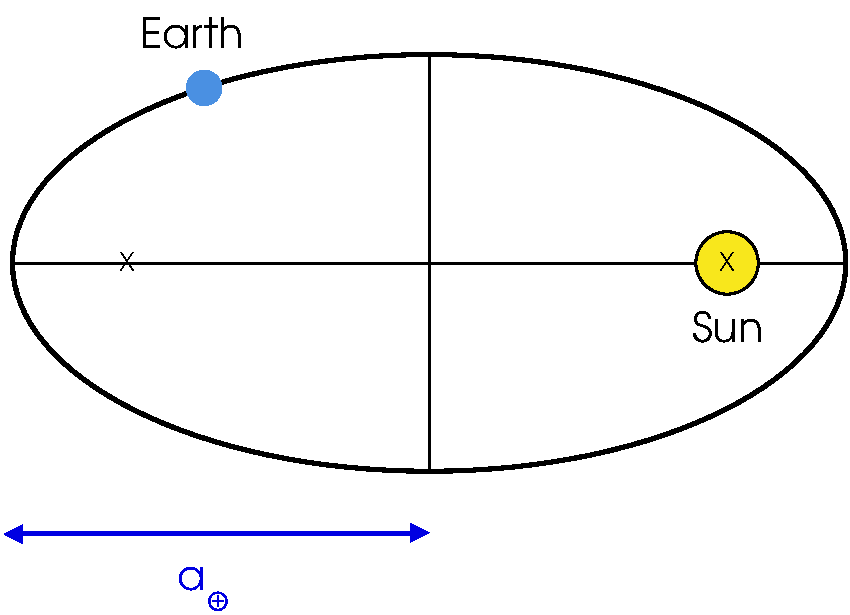
\includegraphics[width=0.60\linewidth]{fig/earth-semi-major-axis}
    \caption{Semi-major axis of Earth's elliptical orbit, used as the characteristic length of the system}
    \label{fig:earth-semi-major-axis}
\end{figure}

Looking at the \(p_j\) from \cref{eq:pr,eq:ptheta,eq:pphi} we can infer their units:

\begin{align}
    k_{pr} &= \frac{k_m}{k_r k_t} \\[0.2cm]
    k_{p\theta} &= \frac{k_m k_r^2}{k_t} = k_{pr} k_r \\[0.2cm]
    k_{p\phi} &= k_{p\theta}
\end{align}

We now introduce the quantity

\begin{equation}
    b_j = \frac{p_j}{m_s}.
\end{equation}
It proves useful to introduce into Hamilton's equations because the mass cancels out (as expected from Newton's 2nd Law, and thus removes the need for introducing  selecting characteristic mass \(k_m\). We will treat the interpretation later. \(b_j\) has units:

\begin{align}
    k_{br} = \frac{k_{pr}}{k_m} = \frac{k_r}{k_t} \\[0.2cm]
    k_{b\theta} = \frac{k_{p\theta}}{k_m} = \frac{k_r^2}{k_t} \\[0.2cm]
    k_{b\phi} = \frac{k_{p\phi}}{k_m} = \frac{k_r^2}{k_t}
\end{align}

For the \(q_j\), \cref{eq:rdot,eq:thetadot,eq:phidot}, we set \(b_j = \frac{p_j}{m_s}\) and nondimensionalize:

\begin{align}
    \od{r}{t} &= \frac{\blue{p_r}}{\blue{p_r}} \\[0.2cm]
    \Leftrightarrow \od{r}{t} &= \blue{b_r} \\[0.2cm]
    \Leftrightarrow \frac{k_r}{k_t} \od{R}{T} &= k_{br} B_r,
\end{align}
so we get
\begin{empheq}[box=\widefbox]{align}
    \label{eq:Rdot}
    \dot{R} = B_r
\end{empheq}

\begin{align}
    \od{\theta}{t} &= \frac{\blue{p_\theta}}{\blue{m_s} r^2} \\[0.2cm]
    \Leftrightarrow \od{\theta}{t} &= \frac{\blue{b_\theta}}{r^2} \\[0.2cm]
    \Leftrightarrow \od{\theta}{t} &= \frac{b_\theta}{r^2} \\[0.2cm]
    \Leftrightarrow \frac{1}{k_t} \od{\theta}{T} &= \frac{k_{b\theta}}{k_r^2} \frac{B_\theta}{R^2},
\end{align}
so we get
\begin{empheq}[box=\widefbox]{align}
    \label{eq:thetadot-nondim}
    \dot{\theta} = \frac{B_\theta}{R^2}
\end{empheq}

\begin{align}
    \od{\phi}{t} &= \frac{\blue{p_\phi}}{{\blue{m_s}} r^2 \sin^2{\theta}} \\[0.3cm]
    \Leftrightarrow \od{\phi}{t} &= \frac{\blue{b_\phi}}{r^2 \sin^2{\theta}}  \\[0.3cm]
    \Leftrightarrow \frac{1}{k_t} \frac{\Phi}{T} &= \frac{k_\phi}{k_r^2} \frac{B_\phi}{R^2 \sin^2{\theta}},
\end{align}
so we get
\begin{empheq}[box=\widefbox]{align}
    \label{eq:phidot-nondim}
    \dot{\phi} = \frac{B_\phi}{R^2 \sin^2{\theta}}
\end{empheq}

For the \(p_j\), \cref{eq:prdot,eq:pthetadot,eq:pphidot} , we first divide by \(m_s\) then set \(b_j = \frac{p_j}{m_s}\) (\blue{relevant terms marked in blue}) and \(\mu_k = G M_k\), and finally nondimensionalize:

\begin{align}
    \begin{split}
        \od{\blue{p_r}}{t} = -\pd{H}{q_r} &= \frac{\blue{p_\theta^2}}{\blue{m_s} r^3} + \frac{\blue{p_\phi^2}}{\blue{m_s} r^3 \sin^2{\theta} } \\
        &+ G \blue{m_s} \sum\limits_{k} M_k \frac{-\left[r - r_k \left(\cos{\theta}\cos{\theta_k} + \sin{\theta}\sin{\theta_k}\cos{(\phi - \phi_k)}\right) \right]}{\left[(r - r_k)^2 \left(\cos{\theta}\cos{\theta_k} + \sin{\theta}\sin{\theta_k}\cos{(\phi - \phi_k)} \right) \right]^{3/2}}
    \end{split} \\[0.3cm]
    \begin{split}
        \Leftrightarrow \od{\blue{b_r}}{t} &= \frac{\blue{b_\theta^2}}{r^3} + \frac{\blue{b_\phi^2}}{r^3 \sin^2{\theta} } \\
        &+ \sum\limits_{k} \mu_k \frac{-\left[r - r_k \left(\cos{\theta}\cos{\theta_k} + \sin{\theta}\sin{\theta_k}\cos{(\phi - \phi_k)}\right) \right]}{\left[(r - r_k)^2 \left(\cos{\theta}\cos{\theta_k} + \sin{\theta}\sin{\theta_k}\cos{(\phi - \phi_k)} \right) \right]^{3/2}}
    \end{split} \\[0.3cm]
    \begin{split}
        \Leftrightarrow \teal{\frac{k_{br}}{k_t}} \od{B_r}{T} &= \orange{\frac{k_{b\theta}^2}{k_r^3}} \frac{B_\theta^2}{R^3} + \orange{\frac{k_{b\phi}^2}{k_r^3}} \frac{B_\phi^2}{R^3 \sin^2{\theta} } \\
        &+ \red{\frac{k_r^3}{k_t^2}\frac{1}{k_r^2}} \sum\limits_{k} \eta_k \frac{-\left[R - R_k \left(\cos{\theta}\cos{\theta_k} + \sin{\theta}\sin{\theta_k}\cos{(\phi - \phi_k)}\right) \right]}{\left[(R - R_k)^2 \left(\cos{\theta}\cos{\theta_k} + \sin{\theta}\sin{\theta_k}\cos{(\phi - \phi_k)} \right) \right]^{3/2}}
    \end{split}
\end{align}

where the characteristic units are colored teal, orange and red, \([\mu] = [G] [M_k] = \frac{k_r^3}{k_m k_t^2} k_m = \frac{k_r^3}{k_t^2} \), the first part of the red factor, the second part being from the fraction inside the summation, having units \(\frac{1}{k_r^2}\). Dividing \(\frac{k_{br}}{k_t}\) over from the left-hand side the units cancel as they must:

\begin{align}
    & \teal{\frac{k_t}{k_{br}}} \orange{\frac{k_{b\theta}^2}{k_r^3} } \\
    = &\frac{k_t^2}{k_r} \frac{k_r^4}{k_t^2 k_r^3}\\
    = &1,
\end{align}
and equivalent same for the second orange since \(k_\theta\) and \(k_\phi\) have the same units. And the red terms:

\begin{align}
    & \teal{\frac{k_t}{k_{br}}} \red{\frac{k_r^3}{k_t^2}\frac{1}{k_r^2}} \\
    = &\frac{k_t^2}{k_r} \frac{k_r^3}{k_t^2} \frac{1}{k_r^2} \\
    = &1
\end{align}

and we are left with the nondimensionalized equation:
\begin{empheq}[box=\widefbox]{align}
    \label{eq:Brdot}
    \dot{B}_r = &\frac{B_\theta^2}{R^3} + \frac{B_\phi^2}{R^3 \sin^2{\theta}} \\
    & + \sum\limits_{k} \eta_k \frac{-\left[R - R_k \left(\cos{\theta}\cos{\theta_k} + \sin{\theta}\sin{\theta_k}\cos{(\phi - \phi_k)}\right) \right]}{\left[(R - R_k)^2 \left(\cos{\theta}\cos{\theta_k} + \sin{\theta}\sin{\theta_k}\cos{(\phi - \phi_k)} \right) \right]^{3/2}} \nonumber
\end{empheq}

The exact same procedure for \(\dot{p_\theta}\) and \(\dot{p}_\phi\) gives us:

\begin{empheq}[box=\widefbox]{align}
    \label{eq:Bthetadot}
    \dot{B}_\theta = &\frac{B_\phi^2}{R^2 \sin^2{\theta} \tan{\theta}} \\
    &+ \sum\limits_{k} \eta_k \frac{R R_k \left[-\sin{\theta}\cos{\theta_k} + \cos{\theta}\sin{\theta_k}\cos{(\phi - \phi_k)} \right]}{\left[(R - R_k)^2 \left(\cos{\theta}\cos{\theta_k} + \sin{\theta}\sin{\theta_k}\cos{(\phi - \phi_k)} \right) \right]^{3/2}} \nonumber
\end{empheq}

\begin{empheq}[box=\widefbox]{align}
    \label{eq:Bphidot}
    \dot{B}_\phi = &\sum\limits_{k} \eta_k \frac{- R R_k \sin{\theta}\sin{\theta_k}\sin{(\phi - \phi_k)}}{\left[(R - R_k)^2 \left(\cos{\theta}\cos{\theta_k} + \sin{\theta}\sin{\theta_k}\cos{(\phi - \phi_k)} \right) \right]^{3/2}}
\end{empheq}

As an overview, \cref{apx:hr4b-overview} shows all six nondimensionalized equations of motion one a single page.

\subsection{H-R4B Numerical Integration Algorithm}

\subsubsection{Symplectic Euler}
In the explicit Euler, all quantities from the Hamiltonian derivative on the right hand refer to the old time step \(i\). In the implicit, they are all referring to the new time step \(i+1\), which results in implicit equations that can typically only be solved numerically.

The symplectic Euler is mixture between explicit and implicit Euler \cite{Hairer}:

\begin{equation}
    \begin{split} \label{eq:symplectic-euler1}
        \vec{q}_{i+1} = \vec{p}_i + h \pd{H}{\vec{p}}(q_i, p_{i+1}) \\
        \vec{p}_{i+1} = \vec{p}_i - h \pd{H}{\vec{q}}(q_i, p_{i+1})
    \end{split}
\end{equation}

or

\begin{equation}
    \begin{split} \label{eq:symplectic-euler2}
        \vec{q}_{i+1} = \vec{p}_i + h \pd{H}{\vec{p}}(q_{i+1}, p_i) \\
        \vec{p}_{i+1} = \vec{p}_i - h \pd{H}{\vec{q}}(q_{i+1}, p_i)
    \end{split}
\end{equation}

One can choose whichever is easier to solve for the equations at hand. We choose \cref{eq:symplectic-euler2} so we get
\begin{align}
    R_{i+1} &= R_i + h B_{r,i} \label{eq:symplectic-euler-R_i+1}, \\[0.4cm]
    \theta_{i+1} &= \theta_i + h \frac{B_{\theta,i}}{R_{i+1}^2}, \label{eq:symplectic-euler-theta_i+1} \\[0.4cm]
    \phi_{i+1} &= \phi_i + h \frac{B_{\phi,i}}{R_{i+1}^2 \sin^2{\theta_{i+1}}}, \label{eq:symplectic-euler-phi_i+1}
\end{align}
\begin{align}    
    \begin{aligned}
        B_{r,i+1} = & B_{r,i} + h \left[ \frac{B_{\theta,i}^2}{R_{i+1}^3} + \frac{B_{\phi,i}^2}{R_{i+1}^3 \sin^2{\theta_{i+1}}} \right. \\
        & \hspace{-22.0pt} + \left. \sum\limits_{k} \eta_k \frac{-\left[R_{i+1} - R_{k,i} \left(\cos{\theta_{i+1}}\cos{\theta_{k,i}} + \sin{\theta_{i+1}}\sin{\theta_{k,i}}\cos{(\phi_{i+1} - \phi_{k,i})}\right) \right]}{\left[(R_{i+1} - R_{k,i})^2 \left(\cos{\theta_{i+1}}\cos{\theta_{k,i}} + \sin{\theta_{i+1}}\sin{\theta_{k,i}}\cos{(\phi_{i+1} - \phi_{k,i})} \right) \right]}^{3/2} \right] , \label{eq:symplectic-euler-Br_i+1}
    \end{aligned} \\[0.4cm]
    \begin{aligned}
        B_{\theta,i+1} = & B_{\theta,i} + h \left[ \frac{B_{\phi,i}^2}{R_{i+1}^2 \sin^2{\theta_{i+1}} \tan{\theta_{i+1}}} \right. \\
        & \hspace{-22.0pt} + \left. \sum\limits_{k} \eta_k \frac{R_{i+1} R_{k,i} \left[-\sin{\theta_{i+1}}\cos{\theta_{k,i}} + \cos{\theta_{i+1}}\sin{\theta_{k,i}}\cos{(\phi_{i+1} - \phi_{k,i})} \right]}{\left[(R_{i+1} - R_{k,i})^2 \left(\cos{\theta_{i+1}}\cos{\theta_{k,i}} + \sin{\theta_{i+1}}\sin{\theta_{k,i}}\cos{(\phi_{i+1} - \phi_{k,i})} \right) \right]^{3/2}} \right], \label{eq:symplectic-euler-Btheta_i+1}
    \end{aligned} \\[0.4cm]
    \begin{aligned}
        B_{\phi,i+1} = & B_{\phi,i} + h \left[ \vphantom{\frac12} \right.\\
        & \hspace{-22.0pt} \hphantom{+} \left. \sum\limits_{k} \eta_k \frac{- R_{i+1} R_{k,i} \sin{\theta_{i+1}}\sin{\theta_{k,i}}\sin{(\phi_{i+1} - \phi_{k,i})}}{\left[(R_{i+1} - R_{k,i})^2 \left(\cos{\theta_{i+1}}\cos{\theta_{k,i}} + \sin{\theta_{i+1}}\sin{\theta_{k,i}}\cos{(\phi_{i+1} - \phi_{k,i})} \right) \right]^{3/2}} \right]. \label{eq:symplectic-euler-Bphi_i+1}
    \end{aligned}
\end{align}
As we can see, we are lucky with this Hamiltonian since we can simply run all steps in the order above, \cref{eq:symplectic-euler-R_i+1,eq:symplectic-euler-theta_i+1,eq:symplectic-euler-phi_i+1,eq:symplectic-euler-Br_i+1,eq:symplectic-euler-Btheta_i+1,eq:symplectic-euler-Bphi_i+1} without needing to solve any implicit equations.
